\documentclass[conference,letterpaper]{IEEEtran}

\usepackage{fontspec}
\usepackage{hyperref}
\usepackage[style=ieee,backend=biber]{biblatex}
\addbibresource{report.bib}

\usepackage{tikz}
\usetikzlibrary{shapes,decorations,arrows,positioning,fit}
\tikzset{point/.style={circle,draw,fill=black,radius=2pt}}
\tikzset{cpoint/.style={circle,draw,fill=white,radius=2pt}}
\tikzset{>=stealth',thick}

\usepackage{fancyhdr}
\usepackage{lastpage}
\usepackage{flushend}
\renewcommand{\headrulewidth}{0pt}
\cfoot{Page {\thepage} {of} {\pageref{LastPage}}}

\title{Multi-Agent Continuous Motion Simulation using Discrete Events}
\author{%
    Jack Rosenthal \\
    Colorado School of Mines \\
    Computer Science Department \\
    \texttt{jrosenth@mines.edu}
    \and
    Qin Yang \\
    Colorado School of Mines \\
    Computer Science Department \\
    \texttt{qinyang@mines.edu}}

\rhead{Rosenthal and Yang, 2018}


\hypersetup{
    pdfauthor={Jack Rosenthal and Qin Yang},
    pdftitle={Multi-Agent Continous Motion Simulation using Discrete Events},
    pdfsubject={Computer Simulation Techniques}
}

\begin{document}

\maketitle
\thispagestyle{fancyplain}
\pagestyle{fancyplain}

\begin{abstract}
    Multi-agent systems with continuous motion (such as swarm robotics systems)
    are often simulated in a time-step agent-based simulation system due to the
    relative ease of implementing an emergent behavior in agent-based
    simulations. The disadvantage of this approach is that simulation accuracy
    is proportional to the size of the time-step in the system, and as the size
    of the time-step decreases, the computational time required to run the
    simulation increases.

    Our paper proposes a modified discrete event simulation technique for
    simulating many agents operating in the same continuous space. We do so by
    adding two new techniques to a discrete event simulation we call
    \emph{cross-cutting} and \emph{cancellation}. We then model the modified
    discrete event simulation using a context-free grammar. Finally, we provide
    an evaluation of the computational complexity of our modified discrete
    event simulation technique when compared to time-step agent-based
    simulations, both theoretically and through an empirical evaluation.
\end{abstract}

\section{Introduction}

Simulating continuous motion of many agents in the same space is non-trivial to
implement, as the motions of one agent may depend on the motions of the
surrounding agents. Often times, the system may be thought of using emergent
behaviors; that is, each agent follows a simple set of rules in order to
accomplish a behavior much greater than the sum of its parts.

Emergent behaviors are easy to implement in a time-step agent-based simulation,
as the individuals behaviors can simply be encoded as a set of predicates and
the resulting transition to the agent at each time step. While this model has
the advantage of easy implementation and trivial verification, it is not very
computationally efficient as the computational time required is proportional to
the amount of steps in the simulation.

Certain multi-agent systems \emph{need} to be encoded using a time-step
agent-based simulation. For example, consider Conway's Game of
Life \cite{conway}, a cellular automaton: each agent fundamentally may only make
a plan for the next step in the simulation by the very nature of the game. But
in some systems, agents may plan for a continuous motion and only adjust their
plan when they need to. For example, a driver of a vehicle may have their
entire route planned ahead of time, but may have to make changes based on their
simple rules for driving on the road (avoid accidents with other vehicles,
don't drive on closed roads, etc.) For the latter kind of simulation, we can
save computational time and improve simulation accuracy by implementing as a
discrete event simulation rather than a time step model, at the cost of reduced
implementation ease, and significantly reduced ease of verifying the
computational model.

This paper extends the traditional discrete event simulation model by adding
two new techniques to support continuous motion simulation with multiple
agents:
\begin{enumerate}
    \item Events may now be \emph{cancelled}. In terms of a typical discrete
        event simulation software system, this means that previously scheduled
        events may be removed from the event queue (or are otherwise prevented
        from being processed) before they are processed.
    \item Events must provide \emph{cross-cutting}. In terms of a typical
        discrete event simulation software system, events which interfere with
        the completion of other events must trigger the cancellation and
        rescheduling to occur.
\end{enumerate}

Our paper implements these techniques for modeling continuous motion of
multiple agents under the following technique:
\begin{enumerate}
    \item When a simulation agent $A$ makes an initial plan, they schedule an
        event $E_{A1}$ indicating the planned time of arrival at the desired
        position and create continuous functions which will represent their
        position and distance traveled with respect to the simulation clock as
        they move to that position.
    \item When a simulation agent $B$ executes an event $E_{B1}$ which
        cross-cuts (prevents) $A$'s plan from completing as intended,
        simulation agent $A$ will devise a new plan, evaluating their
        previously derived continuous position and distance functions, updating
        their distance traveled accordingly, and derives new position and
        distance traveled functions from their previously evaluated position.
        $A$ will then schedule the new event $E_{A2}$ indicating their new plan
        for arrival.
\end{enumerate}
Figure~\ref{fig:introagentfunctions} shows a scenario derived from above
example in a picture.

\begin{figure}[ht]

    \begin{center}
    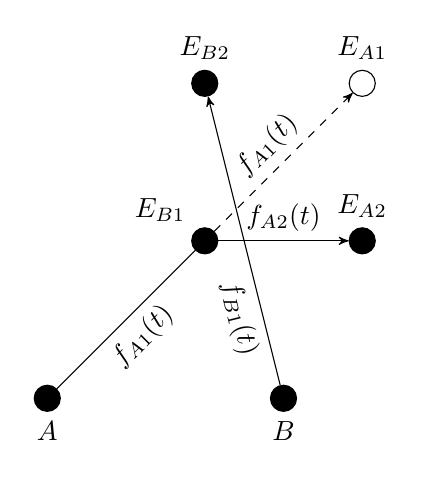
\begin{tikzpicture}
        \node[point,label=below:{$A$}] (Ainitial) at (0,0) {};
        \node[point,label=above left:{$E_{B1}$}] (collide) at (2,2) {};
        \node[cpoint,label={$E_{A1}$}] (EA1) at (4,4) {};
        \node[point,label={$E_{A2}$}] (EA2) at (4,2) {};

        \node[point,label=below:{$B$}] (Binitial) at (3,0) {};
        \node[point,label={$E_{B2}$}] (EB2) at (2,4) {};

        \draw (Ainitial) -- (collide) node[midway,sloped,below] {$f_{A1}(t)$};
        \draw[->,dashed] (collide) -- (EA1) node[midway,sloped,above] {$f_{A1}(t)$};
        \draw[->] (collide) -- (EA2) node[midway,sloped,above] {$f_{A2}(t)$};
        \draw[->] (Binitial) -- (EB2) node[near start,sloped,below] {$f_{B1}(t)$};
    \end{tikzpicture}
    \end{center}

    \caption{Initially, agent $A$ plans on arrival at the point indicated by
    $E_{A1}$ with continuous travel function $f_{A1}(t)$. Then, agent $B$
    schedules travel to the point indicated by $E_{B2}$, but realizes this will
    cause collision with $A$, and $A$ would notice this at time $t_c$. $B$ then
    schedules $E_{B1}$ for time $t_c$ to indicate to $A$ to change the plan of
    travel. When $E_{B1}$ is executed, $A$ then evaluates $f_{A1}(t_c)$ to
    determine its position, and creates a new travel function $f_{A2}(t)$
    indicating the planned travel to the point indicated by $E_{A2}$.
    Presumably, at this point $A$ may wish to schedule another event to reach
    its initial desired position.}
    \label{fig:introagentfunctions}

\end{figure}

Finally, we show how this modified kind of discrete event simulation can be
modeled using a context-free grammar.

The remainder of the paper is organized as follows...

\section{Related Work}

Swarm robotics in a new and rising field, and many simulators for swarm
robotics systems have been developed. For example, ARGoS \cite{argos}, Gazebo
\cite{gazebo}, USARSim \cite{usarsim}, Webots \cite{webots}, and MuRoSimF
\cite{murosimf} are all simulators for multi-robot systems. However, all of
these simulators use a time-step agent-based model for their simulations. Our
computational model is implemented using a discrete event simulation (see
\cite[p.~3]{leemispark} for the definition of a discrete event simulation),
which is a fundamentally different simulation model than all of the previously
mentioned simulators.

\section{Problem Description}

Describe with technical detail / math the problem that you are solving.  What
information is given, and what are you trying to find?  Equivalently, what are
the inputs and outputs of your algorithm?  Describe the technical challenges
for this work.

\section{Method (/ Algorithm)}

Describe with technical detail / math / pseudocode how your solution works.
Block diagrams are often helpful, either here or in the problem description.

\section{Results / (Experiments/Evaluation)}


Describe the performance of method / algorithm / implementation.
Explain your experimental setup: hardware / software versions, test
problems, and metrics.  Present results for each test.  Plots and
tables are often helpful to present the results.  Explain and
interpret the results.  Where they as expected?  Why did the approach
perform as observed?

\section{Conclusion}

In a few paragraphs, summarize all of the above sections.  Emphasize especially
any novel contribution of your project.  Give any final thoughts on challenges
faced, lessons learned, and future steps for the work.

\printbibliography

\end{document}
